\documentclass[10pt]{article}

% ---------- Packages ----------
\usepackage[letterpaper, margin=1in, headheight=14pt]{geometry}
\usepackage[T1]{fontenc}
\usepackage{lmodern}
\usepackage{textcomp}
\usepackage{amsmath}
\usepackage{graphicx}
\usepackage{booktabs}
\usepackage{tabularx}
\usepackage{longtable}
\usepackage{array}
\usepackage{float}
\usepackage{caption}
\usepackage{enumitem}
\usepackage{titlesec}
\usepackage{xcolor}
\usepackage[hidelinks]{hyperref}

\graphicspath{{../results/plots/}}
\setlength{\parindent}{0pt}
\setlength{\parskip}{5pt}
\renewcommand{\arraystretch}{1.15}
\newcolumntype{L}{>{\raggedright\arraybackslash}X}
\setlist{itemsep=2pt, topsep=3pt}
\captionsetup{font=small, labelfont=bf}

% ---------- Headings: small caps sections, as in the template ----------
\titleformat{\section}{\Large\scshape}{}{0pt}{}[\vspace{-2pt}]
\titleformat{\subsection}{\large\bfseries}{}{0pt}{}
\titleformat{\subsubsection}{\normalsize\bfseries}{}{0pt}{}
\titlespacing*{\section}{0pt}{16pt}{6pt}
\titlespacing*{\subsection}{0pt}{10pt}{3pt}
\titlespacing*{\subsubsection}{0pt}{8pt}{2pt}

% ---------- Running header: section name left, page number right ----------
\makeatletter
\renewcommand{\sectionmark}[1]{\markboth{#1}{#1}}
\def\ps@report{%
  \def\@oddhead{\vbox{\hbox to\textwidth{\footnotesize\scshape\rightmark\hfil\upshape\thepage}%
    \vskip 2pt\hrule height 0.4pt}}%
  \def\@oddfoot{}\def\@evenhead{\@oddhead}\def\@evenfoot{}}
\makeatother
\pagestyle{report}

\newcommand{\ua}{\,\textmu A}
\newcommand{\pct}{\,\%}

\begin{document}

% ==================================================================
% TITLE PAGE
% ==================================================================
\begin{titlepage}
\centering
\vspace*{3cm}
\rule{\textwidth}{0.6pt}\\[14pt]
{\LARGE COURSE PROJECT}\\[6pt]
{\LARGE DIGITAL VLSI DESIGN}\\[10pt]
\rule{\textwidth}{0.6pt}

\vspace{1.5cm}
{\Large\bfseries ML-Driven PVT Variation Aware Leakage Estimation}\\[14pt]
{\bfseries November 15, 2026}

\vspace{3cm}
{\large Submitted by}\\[10pt]
Jayakanth M V (2025122004)\\[2pt]
Tushar Gupta (2025122001)\\[2pt]
Dhanika Kothari (2024102011)\\[2pt]
Kavya Veer (2024112002)

\vfill
\end{titlepage}

% ==================================================================
\section{Setup}
% ==================================================================

\begin{table}[H]
\centering
\begin{tabularx}{\textwidth}{@{}p{3.2cm}L@{}}
\toprule
Item & Value \\
\midrule
Model file & PTM 32\,nm LP (\texttt{models/32nm\_LP.pm}, BSIM4) \\
Nominal VDD & 1.0\,V (sampled within $\pm$10\pct) \\
Channel length & 32\,nm; widths 1 to 8 $\times$ L$_{\min}$ (32 to 256\,nm) \\
Test circuit & 3-bit carry-lookahead adder (CLA) \\
Simulator & ngspice-44.2 (Windows, batch mode), DC operating-point analysis \\
Software & Python 3.10/3.11, NumPy, pandas, scikit-learn, XGBoost, Matplotlib \\
Netlist options & \texttt{.options gmin=1e-18 abstol=1e-18 reltol=1e-6 vntol=1e-9} in every netlist \\
\bottomrule
\end{tabularx}
\end{table}

\subsubsection*{Summary of results}

\begin{table}[H]
\centering
\small
\begin{tabularx}{\textwidth}{@{}c L r c c c@{}}
\toprule
Part & What is compared & Points & Median error & 95th-pct error & Mean accuracy \\
\midrule
A & Transistor $I_d, I_g, I_s, I_b$ in the ON cases (test set) & 1,500 per case & 0.12--0.59\pct & 1.1--2.8\pct & 99.1--99.7\pct \\
A & Transistor $I_d, I_s, I_b$ in the OFF cases (test set) & 1,500 per case & 0.01--0.15\pct & 0.3--3.2\pct & 99.3--99.9\pct \\
A & Transistor $I_g$ in the OFF cases ($\approx$1e-22\,A, test set) & 1,500 per case & 1.3--4.9\pct & 8.7--22.8\pct & 92.2--97.7\pct \\
B & Leakage of INV, NAND2, NOR2, AND2, OR2 & 3,600 & 0.69\pct & 2.07\pct & 99.17\pct \\
C & Leakage of the 3-bit CLA & 25,600 & 0.74\pct & 1.79\pct & 99.20\pct \\
\bottomrule
\end{tabularx}
\end{table}

All 3,600 gate simulations and all 25,600 circuit operating points are used; none are dropped.
The OFF-state gate current is listed separately because it is about $10^{-22}$\,A and has no
effect on the leakage of any gate or circuit (Section ``Error analysis'').

% ==================================================================
\section{Data generation}
% ==================================================================

\subsection*{Sampling}

For each of the four cases (NMOS ON, NMOS OFF, PMOS ON, PMOS OFF), 10,000 samples are drawn with a
fixed seed per case. VDD is drawn first. The gate and body voltages are fixed by the case.

\begin{table}[H]
\centering
\begin{tabularx}{\textwidth}{@{}p{4.2cm}L@{}}
\toprule
Parameter & Distribution \\
\midrule
VDD & uniform, 0.9 to 1.1\,V \\
$V_d$, $V_s$ & uniform, 0 to VDD (see the two additions below) \\
$W$ & uniform, 32 to 256\,nm \\
Temperature & uniform, $-40$ to 125\,\textdegree C (see below) \\
\texttt{vth0, toxe, ndep, u0, xj} & uniform, model-card value $\pm$10\pct, separate values for NMOS and PMOS \\
\midrule
$V_g$, $V_b$ & NMOS ON: VDD, 0 \quad NMOS OFF: 0, 0 \quad PMOS ON: 0, VDD \quad PMOS OFF: VDD, VDD \\
\bottomrule
\end{tabularx}
\end{table}

Two additions to plain uniform sampling:
\begin{enumerate}
\item \textbf{Mild corner enrichment.} With probability 4\pct\ the temperature is drawn within
10\,\textdegree C of one end of its range, and with probability 6\pct\ $V_d$ (or $V_s$) is drawn
within 5\pct\ of VDD of a rail. This raises the share of samples at the temperature extremes from
12.1\pct\ to about 15.7\pct.
\item \textbf{Gate operating points (20\pct\ of the samples).} Inside a logic gate a transistor is
never at a random $(V_d, V_s)$. OFF transistors sit exactly on the rails, ON transistors have $V_d$
within nanovolts to microvolts of $V_s$, and stack nodes sit a few millivolts from a rail. For
20\pct\ of the samples, $(V_d, V_s)$ is drawn from such points: one terminal at 0\,V, at VDD or
uniform; the other exactly on a rail, within a step $\delta$ of the first terminal, within
$\delta$ of a rail, or uniform, with $\delta$ log-uniform from $10^{-8}$\,V to 0.3\,V. All other
parameters of these samples are drawn as usual.
\end{enumerate}

The second addition was needed for Part B. Models trained without it reached about 1\pct\ error on
their own test set but 20--60\pct\ error inside gates, because the gate operating points lie on
the edge of the sampled region where almost no training samples fall. This is a deliberate
departure from purely uniform $(V_d, V_s)$ sampling; every other parameter is drawn exactly as the
specification asks.

\subsection*{Netlists}

Each sample is one single-transistor netlist in which every terminal has its own voltage source.
The five process parameters are \texttt{.param} variables in a parametrised copy of the model card
(\texttt{32nm\_LP\_param.lib}), and the temperature is set with \texttt{.temp}. Terminal currents
are taken as the current into the device, $-I(V_\text{source})$. Many netlists are run in one
ngspice process, and several processes run in parallel; the 40,000 samples take about 3 minutes.
All 40,000 converged.

Alongside the four terminal currents, the script saves the internal BSIM4 current components of
every sample (channel current, junction currents, gate tunnelling parts, GIDL, impact ionisation).
These are used only as training targets. Example netlists are in \texttt{netlists/transistor},
\texttt{netlists/gates} and \texttt{netlists/circuit}.

\subsection*{Split}

Each dataset is split at random into 7,000 training, 1,500 validation and 1,500 test samples
(70:15:15, seed 42).

\subsection*{Data check}

\textbf{Kirchhoff check} ($I_d + I_g + I_s + I_b$):

\begin{table}[H]
\centering
\begin{tabular}{@{}lccc@{}}
\toprule
Case & Largest residual (A) & Median residual (A) & Median largest terminal current (A) \\
\midrule
NMOS ON  & 2.3e-15 & 1.3e-16 & 2.6e-06 \\
NMOS OFF & 4.8e-22 & 3.5e-26 & 1.7e-14 \\
PMOS ON  & 5.5e-16 & 3.3e-17 & 1.6e-06 \\
PMOS OFF & 1.0e-15 & 3.7e-17 & 1.4e-14 \\
\bottomrule
\end{tabular}
\end{table}

The residuals are at the rounding level of the simulator (about $10^{-16}$\,A), far below the
currents.

\textbf{Trend plots} (Figure~\ref{fig:trends}). The OFF current rises steeply with temperature and
falls with \texttt{vth0} (subthreshold conduction), and the gate current falls steeply as
\texttt{toxe} increases (direct tunnelling), as expected.

\begin{figure}[H]
\centering
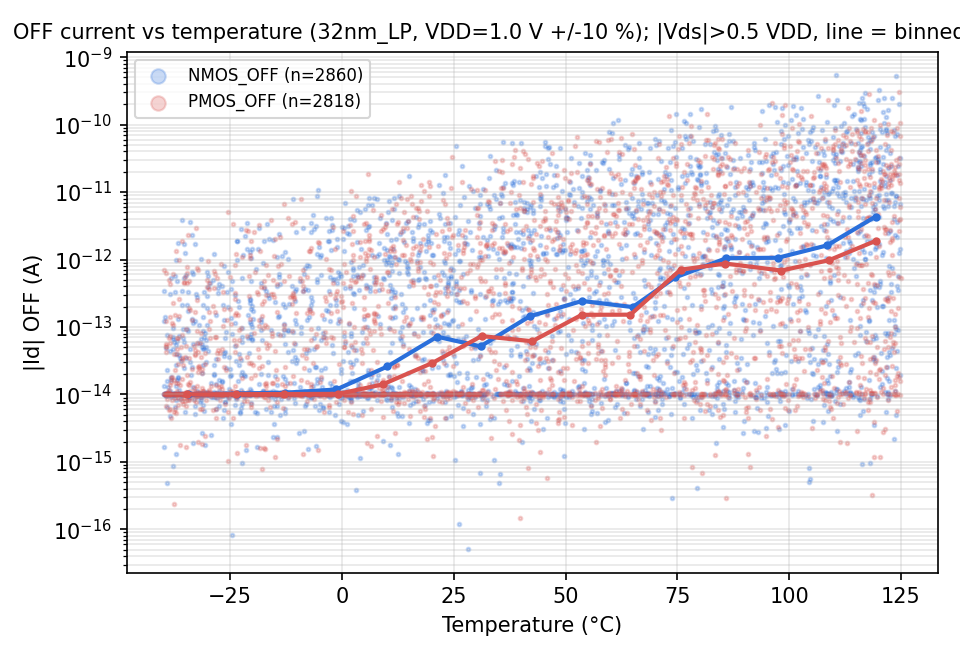
\includegraphics[width=0.49\textwidth]{trend_off_current_vs_temp.png}\hfill
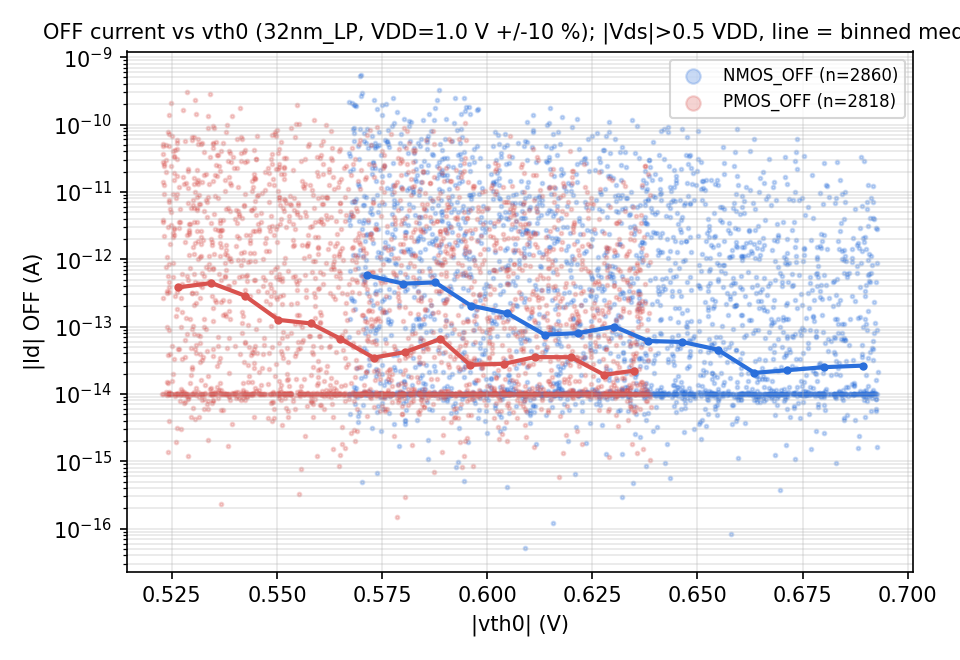
\includegraphics[width=0.49\textwidth]{trend_off_current_vs_vth0.png}\\[4pt]
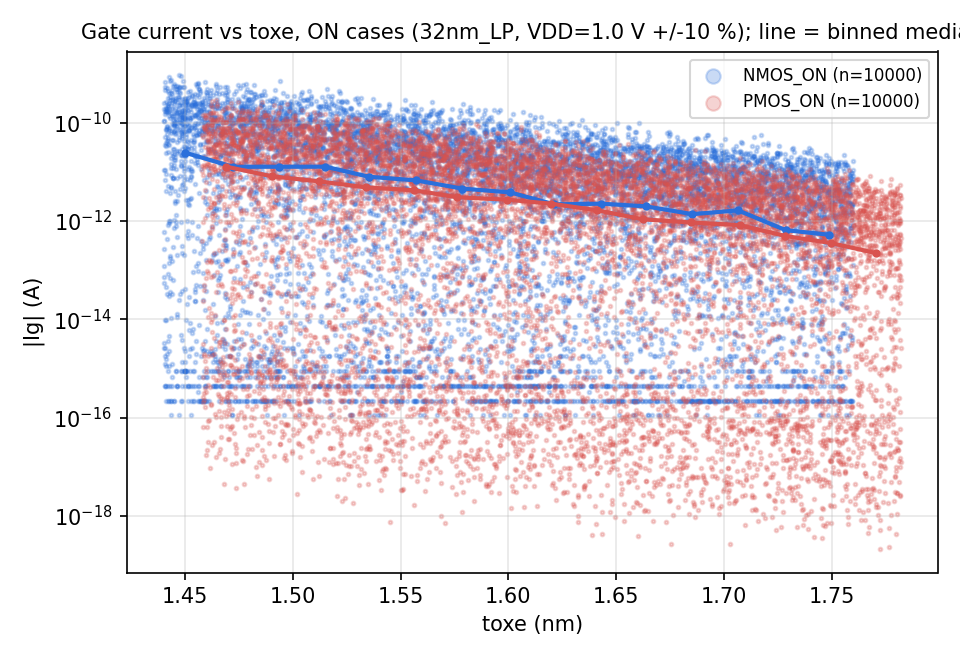
\includegraphics[width=0.49\textwidth]{trend_gate_current_vs_toxe.png}
\caption{Trend plots: OFF current against temperature (top left) and \texttt{vth0} (top right),
and gate current against \texttt{toxe} (bottom).}
\label{fig:trends}
\end{figure}

% ==================================================================
\section{Models}
% ==================================================================

\subsection*{Preprocessing: physics-based component models}

A terminal current is a sum of mechanisms with very different behaviour, so the models do not
learn $I_d$, $I_g$, $I_s$ and $I_b$ directly. Each mechanism gets a physics equation whose
coefficients are fitted on the training set, and the ML model learns only the correction
$\ln(I_\text{SPICE} + \varepsilon) - \ln(I_\text{physics} + \varepsilon)$.

\begin{table}[H]
\centering
\small
\begin{tabularx}{\textwidth}{@{}p{4.3cm}Lc@{}}
\toprule
Mechanism & Physics equation & ML correction \\
\midrule
Channel current, ON & EKV equation with $V_{th}$ including body effect, DIBL, temperature and process & yes \\
Channel current, OFF & subthreshold equation $I_0 (W/L)\, e^{(V_{gs}-V_{th})/nV_t}(1-e^{-V_{ds}/V_t})$ & yes \\
Source junction & reverse diode with the BSIM4 temperature law & yes \\
Gate-body tunnelling & direct-tunnelling form in $W$, \texttt{toxe}, $V_{gb}$, $T$ & yes \\
Gate-channel tunnelling (source and drain side) & same form with $V_{gs}$ and $V_{gd}$ & yes \\
Impact ionisation & function of channel current and $V_{ds}$ & yes \\
Drain junction & diode with $10^{-14}$\,A saturation current (exact) & no \\
GIDL / GISL & BSIM4 GIDL equation with the model-card constants (exact) & no \\
\bottomrule
\end{tabularx}
\end{table}

The four terminal currents are assembled from the mechanisms with Kirchhoff's law, so they always
sum to zero. Other preprocessing:
\begin{itemize}
\item \textbf{Inputs:} 25 features (voltages relative to source and body, temperature terms,
normalised process parameters) plus the six physics-equation values, 31 inputs in total.
\item \textbf{Soft floor $\varepsilon$:} $10^{-5}$ of each mechanism's 90th-percentile magnitude.
Currents far below it are negligible, and the floor stops them from dominating the fit.
\item \textbf{Input limits:} each input is limited to its training range, so a transistor exactly
on a rail cannot push the correction outside what was learned.
\end{itemize}

\subsection*{Model types}

\begin{table}[H]
\centering
\begin{tabularx}{\textwidth}{@{}p{3.4cm}L@{}}
\toprule
Model & Main hyperparameters \\
\midrule
Polynomial ridge & all degree-3 terms of the 31 standardised inputs, ridge $\alpha = 10^{-3}$ \\
Random forest & 300 trees, \texttt{max\_features} 0.5 \\
XGBoost & learning rate 0.03, depth 6, subsample and colsample 0.8, early stopping on 10\pct\ of the training set \\
MLP neural network & 3 hidden layers of 128 (tanh), Adam, learning rate $10^{-3}$, batch 64, early stopping on 10\pct\ of the training set \\
\bottomrule
\end{tabularx}
\end{table}

\subsection*{Model comparison (validation set)}

Error $= |I_\text{ML} - I_\text{SPICE}| / \max(|I_\text{SPICE}|, 1\,\text{fA})$. For the OFF-state
gate current (about $10^{-22}$\,A) the floor is a tenth of its median. $R^2$ is computed on
$\operatorname{asinh}(I/\text{floor})$. Each cell is $R^2$ / median error\pct\ / 95th-percentile
error\pct. The chosen model for each case is in bold.

{\footnotesize
\setlength{\tabcolsep}{2.5pt}
\begin{longtable}{@{}llccccc@{}}
\toprule
Case & Model & $I_d$ & $I_g$ & $I_s$ & $I_b$ & Score \\
\midrule
\endhead
NMOS ON & Polynomial ridge & 1.0000 / 0.40 / 2.05 & 1.0000 / 1.06 / 5.71 & 1.0000 / 0.44 / 2.07 & 0.9999 / 0.35 / 2.15 & 1.78 \\
 & Random forest & 1.0000 / 2.43 / 11.32 & 0.9996 / 4.78 / 19.49 & 1.0000 / 2.44 / 10.98 & 0.9996 / 0.29 / 8.32 & 7.50 \\
 & XGBoost & 1.0000 / 1.17 / 5.56 & 0.9999 / 2.22 / 9.91 & 1.0000 / 1.17 / 5.61 & 0.9999 / 0.23 / 4.65 & 3.81 \\
 & \textbf{MLP} & 1.0000 / 0.53 / 2.51 & 1.0000 / 0.57 / 2.45 & 1.0000 / 0.53 / 2.38 & 1.0000 / 0.12 / 1.12 & \textbf{1.28} \\
\midrule
NMOS OFF & Polynomial ridge & 1.0000 / 0.01 / 1.36 & 0.9912 / 3.68 / 33.07 & 1.0000 / 0.25 / 2.01 & 1.0000 / 0.02 / 1.64 & 5.25 \\
 & Random forest & 0.9999 / 0.02 / 7.02 & 0.9894 / 11.31 / 49.46 & 0.9999 / 0.15 / 6.65 & 1.0000 / 0.01 / 0.21 & 9.35 \\
 & XGBoost & 1.0000 / 0.01 / 3.22 & 0.9975 / 4.85 / 26.18 & 1.0000 / 0.14 / 3.22 & 1.0000 / 0.01 / 0.22 & 4.73 \\
 & \textbf{MLP} & 1.0000 / 0.01 / 1.27 & 0.9968 / 4.63 / 22.95 & 1.0000 / 0.13 / 1.26 & 1.0000 / 0.01 / 0.33 & \textbf{3.82} \\
\midrule
PMOS ON & Polynomial ridge & 1.0000 / 0.27 / 1.42 & 1.0000 / 0.79 / 5.27 & 1.0000 / 0.31 / 1.68 & 1.0000 / 0.25 / 1.78 & 1.47 \\
 & Random forest & 1.0000 / 2.03 / 8.59 & 0.9997 / 3.69 / 15.26 & 0.9997 / 2.03 / 8.62 & 0.9997 / 0.26 / 7.93 & 6.05 \\
 & XGBoost & 1.0000 / 0.97 / 4.67 & 0.9999 / 1.82 / 7.92 & 1.0000 / 0.96 / 4.84 & 0.9999 / 0.15 / 3.67 & 3.13 \\
 & \textbf{MLP} & 1.0000 / 0.32 / 1.51 & 1.0000 / 0.60 / 2.55 & 1.0000 / 0.33 / 1.64 & 1.0000 / 0.14 / 1.08 & \textbf{1.02} \\
\midrule
PMOS OFF & Polynomial ridge & 1.0000 / 0.01 / 1.18 & 0.8856 / 3.95 / 37.47 & 1.0000 / 0.22 / 1.93 & 1.0000 / 0.02 / 1.61 & 5.80 \\
 & Random forest & 0.9999 / 0.01 / 6.37 & 0.9989 / 3.59 / 15.78 & 0.9989 / 0.15 / 6.11 & 1.0000 / 0.01 / 0.30 & 4.04 \\
 & \textbf{XGBoost} & 1.0000 / 0.01 / 2.76 & 0.9997 / 1.26 / 8.51 & 0.9999 / 0.13 / 2.87 & 1.0000 / 0.01 / 0.27 & \textbf{1.98} \\
 & MLP & 1.0000 / 0.01 / 0.98 & 0.9991 / 3.69 / 12.38 & 1.0000 / 0.09 / 0.97 & 1.0000 / 0.01 / 0.31 & 2.30 \\
\bottomrule
\end{longtable}
}

\textbf{Choice.} The score is the mean over the four currents of (median + 95th percentile)\,/\,2,
and the model with the lowest validation score is chosen for each case: the MLP for NMOS ON, NMOS
OFF and PMOS ON, and XGBoost for PMOS OFF. The MLP gives the smoothest corrections, which suits the
smooth physics. XGBoost wins PMOS OFF because of the gate current there. The physics equations
alone score 39 to 54 on the ON cases, so both the physics and the ML correction are needed.

\subsection*{Chosen models on the test set}

Median / 95th-percentile error (\%) on the 1,500 test samples of each case:

\begin{table}[H]
\centering
\begin{tabular}{@{}lcccc@{}}
\toprule
Case & $I_d$ & $I_g$ & $I_s$ & $I_b$ \\
\midrule
NMOS ON (MLP) & 0.53 / 2.77 & 0.59 / 2.68 & 0.53 / 2.59 & 0.12 / 1.19 \\
NMOS OFF (MLP) & 0.01 / 1.12 & 4.88 / 22.80 & 0.12 / 1.11 & 0.01 / 0.34 \\
PMOS ON (MLP) & 0.32 / 1.56 & 0.56 / 2.49 & 0.34 / 1.55 & 0.16 / 1.15 \\
PMOS OFF (XGBoost) & 0.01 / 2.90 & 1.31 / 8.75 & 0.15 / 3.18 & 0.01 / 0.28 \\
\bottomrule
\end{tabular}
\end{table}

The four saved models are \texttt{ml\_models/<CASE>.joblib}. Figure~\ref{fig:predvsspice} shows
the predicted against SPICE currents on the test set.

\begin{figure}[H]
\centering
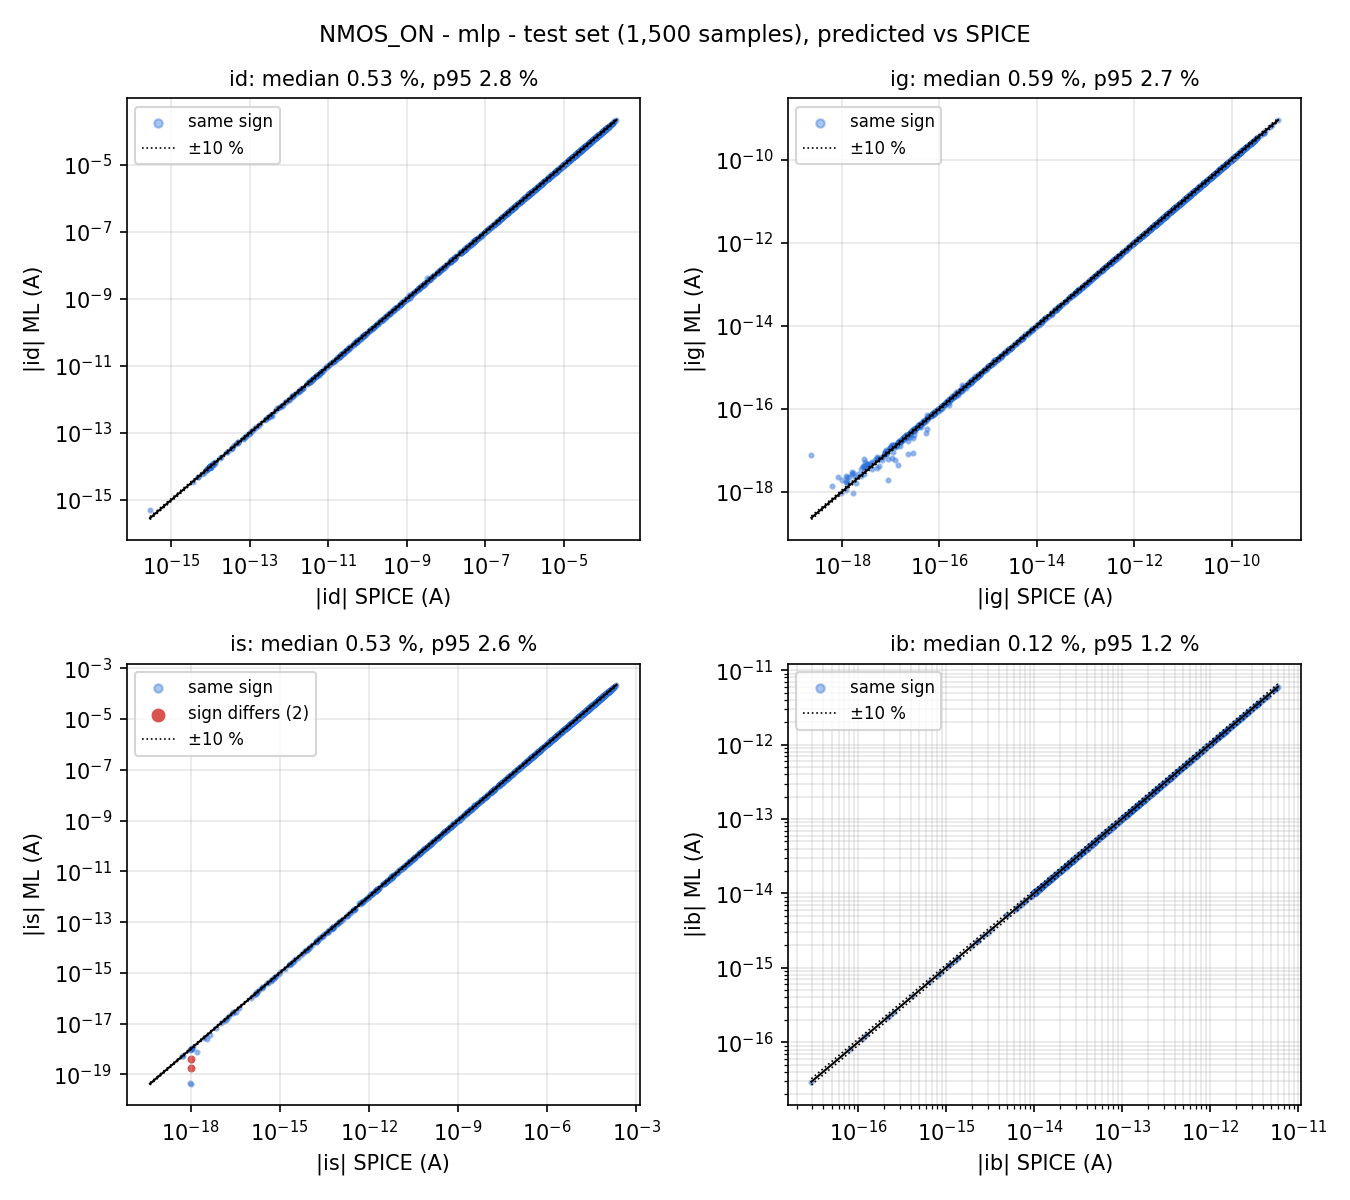
\includegraphics[width=0.49\textwidth]{pred_vs_spice_NMOS_ON.png}\hfill
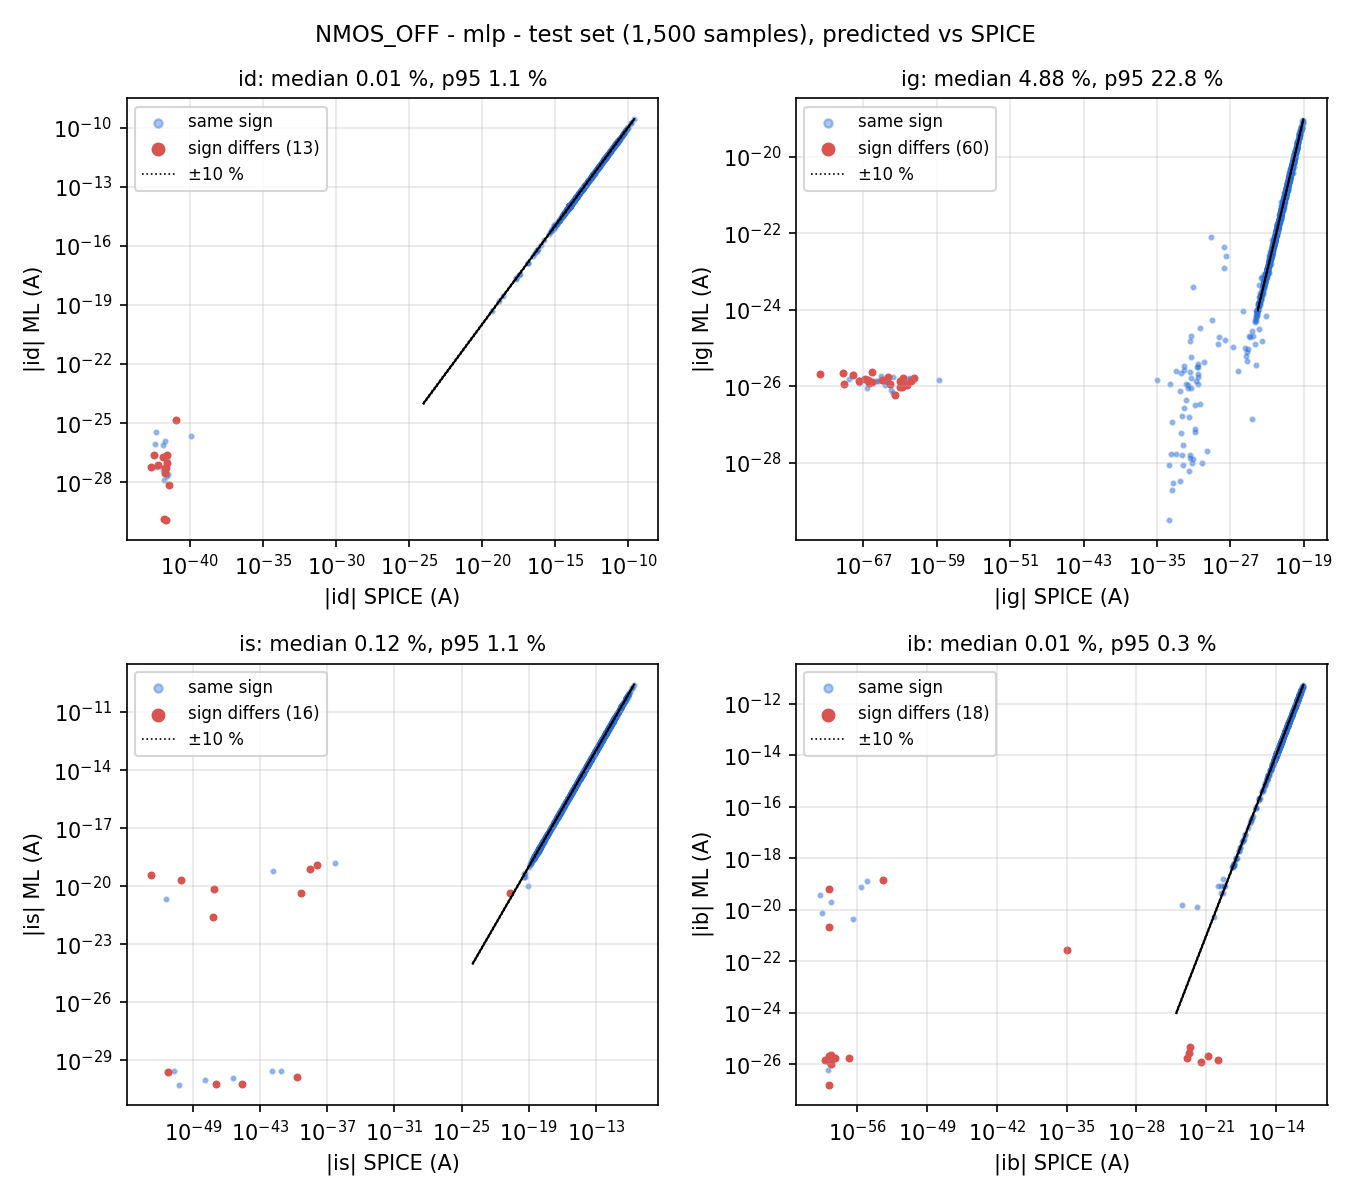
\includegraphics[width=0.49\textwidth]{pred_vs_spice_NMOS_OFF.png}\\[4pt]
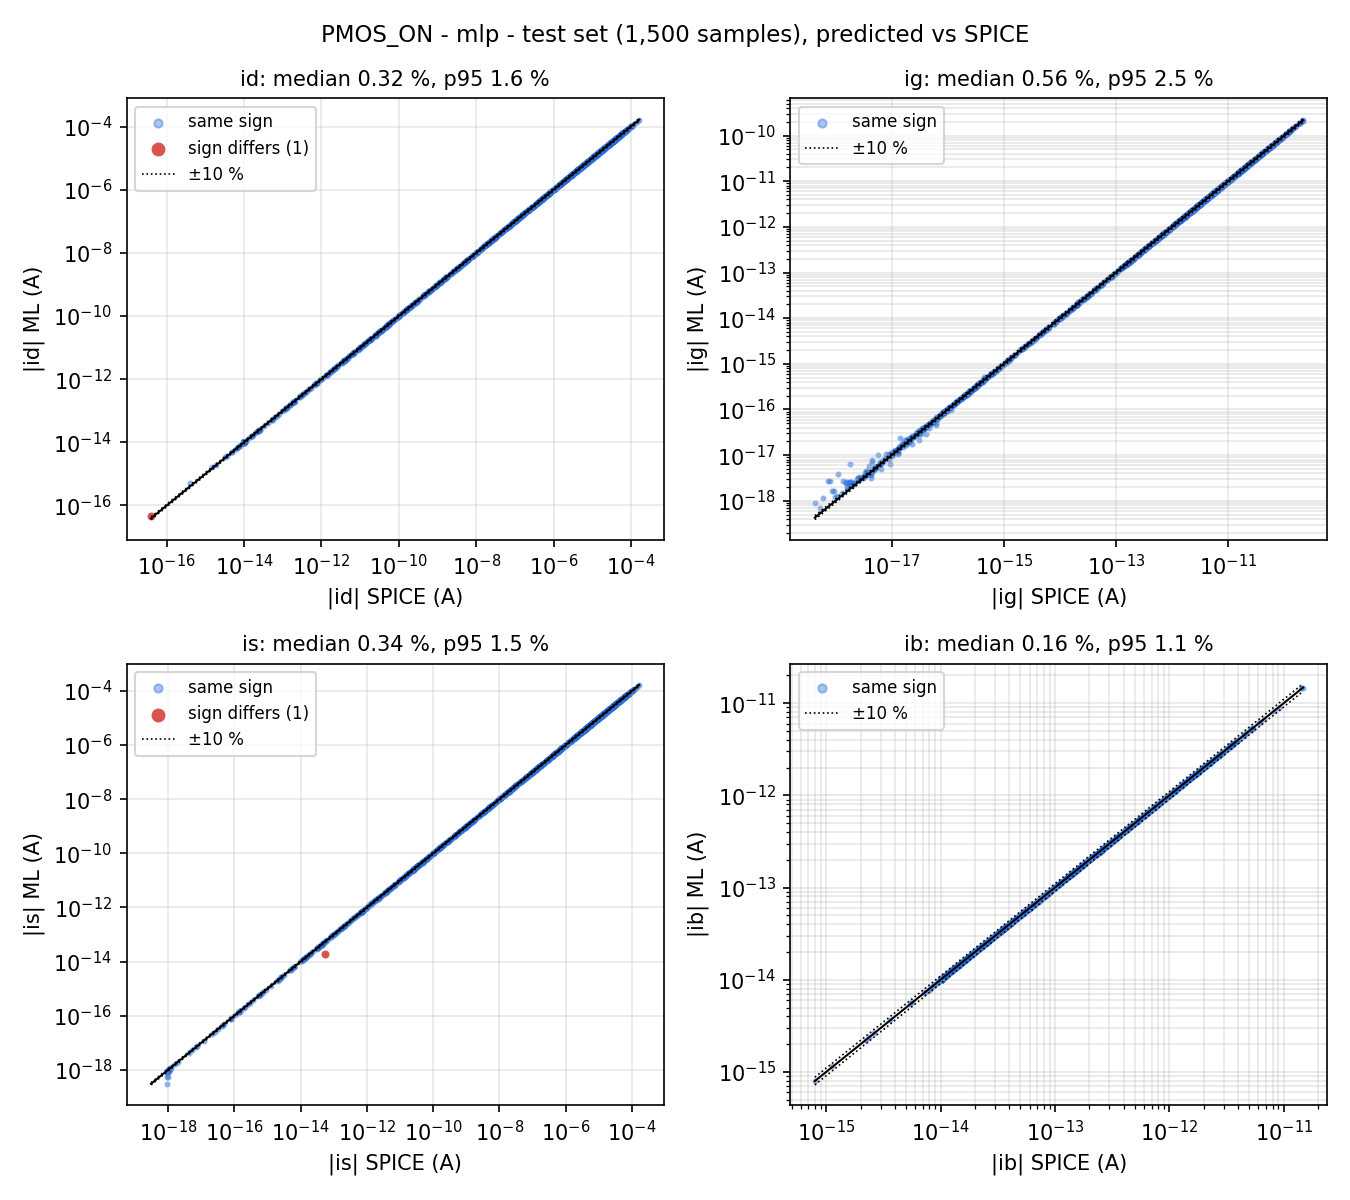
\includegraphics[width=0.49\textwidth]{pred_vs_spice_PMOS_ON.png}\hfill
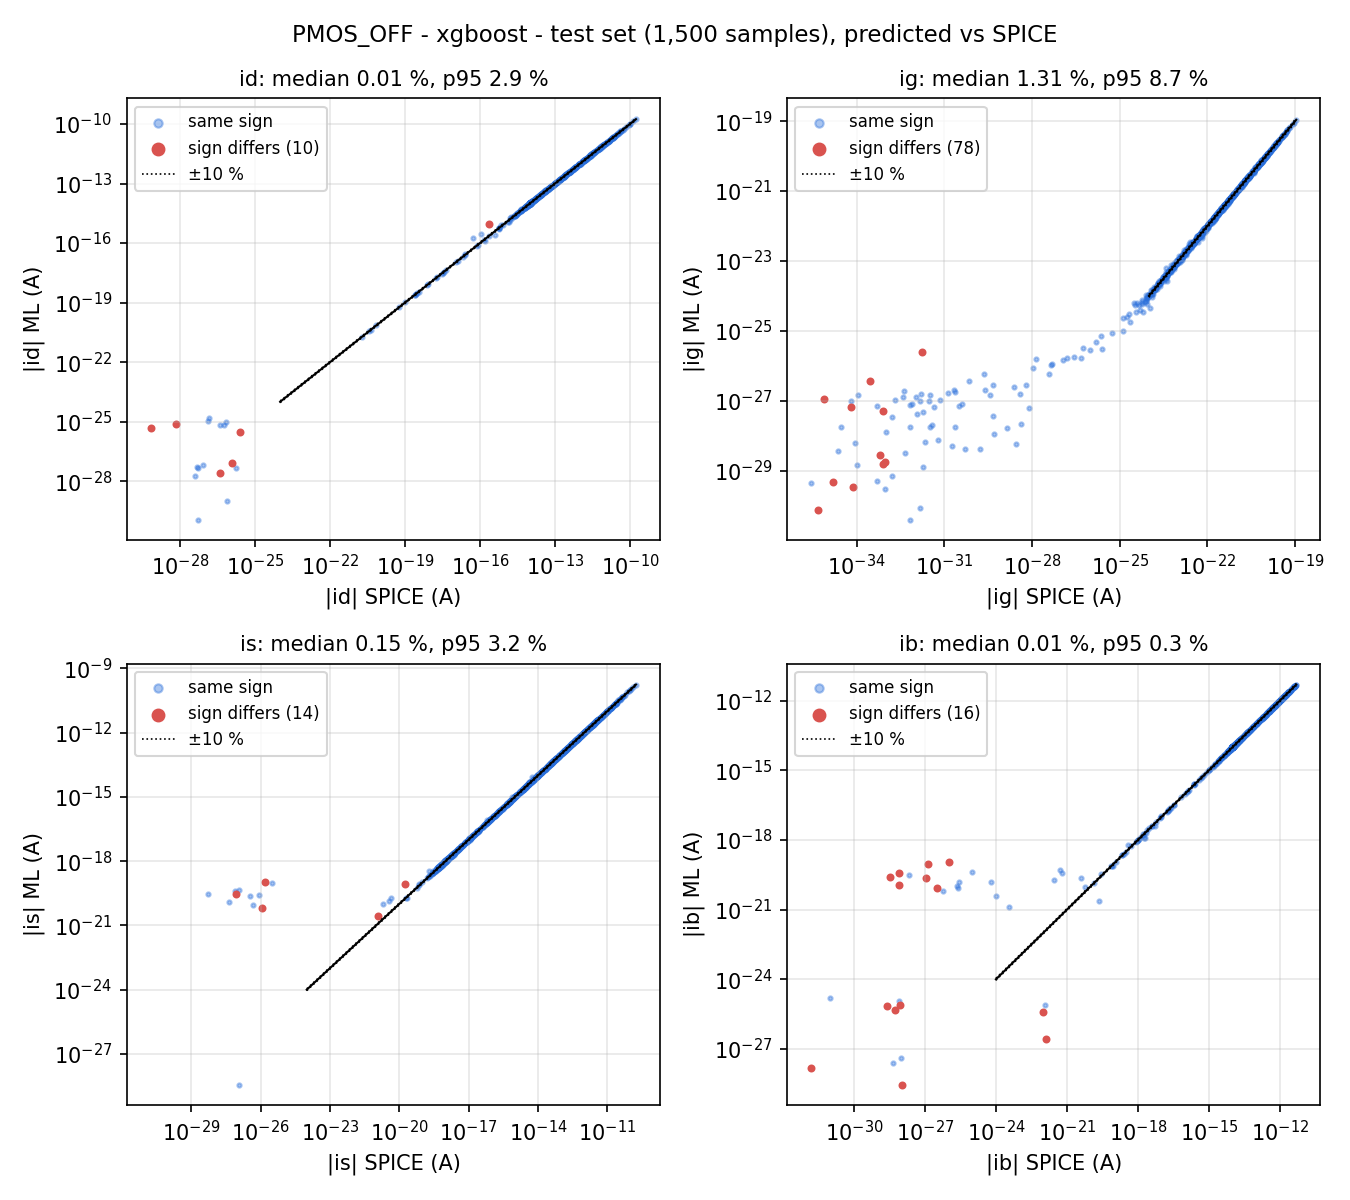
\includegraphics[width=0.49\textwidth]{pred_vs_spice_PMOS_OFF.png}
\caption{Predicted against SPICE terminal currents of the chosen models on the test set: NMOS ON,
NMOS OFF (top), PMOS ON, PMOS OFF (bottom).}
\label{fig:predvsspice}
\end{figure}

% ==================================================================
\section{Gate results}
% ==================================================================

\subsection*{Method}

\begin{itemize}
\item \textbf{Gates:} static CMOS INV, NAND2 and NOR2; AND2 and OR2 are a NAND2 or NOR2 followed
by an INV and are simulated as complete gates. Widths (NMOS / PMOS, in L$_{\min}$): INV 2 / 4,
NAND2 4 / 4, NOR2 2 / 8. Input order is AB; in the NAND2, A drives the NMOS next to the output,
and in the NOR2, A drives the PMOS next to VDD.
\item \textbf{Corners:} 200 random draws of VDD, temperature and the ten process parameters (seed
2025). All NMOS in a gate share one process draw and all PMOS another. Inputs are at exactly 0 or
VDD.
\item \textbf{SPICE reference:} all 18 cases at all 200 corners, 3,600 simulations. A solution is
accepted only if it converged and every node lies within $[0, \text{VDD}]$. Otherwise the
simulation is rerun with a different starting guess and, as a last resort, with ngspice's KLU
solver (\texttt{.options klu}). Four simulations needed a rerun and all 3,600 give a usable
solution. These results are used only for evaluation, never for training.
\item \textbf{Leakage:} the current drawn from every source at VDD (the supply and the inputs that
are high), which equals the static power divided by VDD.
\item \textbf{ML prediction:} the internal node and output voltages recorded from SPICE give the
terminal voltages of each transistor. The ON or OFF model of Part A predicts its terminal
currents, and the gate leakage is $\sum (V_d I_d + V_g I_g + V_s I_s + V_b I_b) / \text{VDD}$ over
the transistors.
\item \textbf{Internal node voltages from ML:} also recorded, by solving Kirchhoff's current law at
each internal node with the transistor models. They agree with SPICE to a few microvolts, and the
leakage computed from them has the same accuracy (median 0.70\pct, 95th percentile 2.07\pct).
\end{itemize}

\subsection*{Gate results table}

\begin{table}[H]
\centering
\small
\begin{tabular}{@{}llcccccc@{}}
\toprule
Gate & Input & SPICE median (A) & ML median (A) & Bias\,\% & Median err.\,\% & p95 err.\,\% & Mean err.\,\% \\
\midrule
INV & 0 & 2.137e-11 & 2.133e-11 & 0.53 & 0.78 & 2.30 & 0.90 \\
INV & 1 & 4.278e-11 & 4.257e-11 & 0.26 & 0.68 & 2.60 & 0.91 \\
\midrule
NAND2 & 00 & 2.522e-11 & 2.495e-11 & 0.56 & 0.78 & 2.52 & 0.97 \\
NAND2 & 01 & 9.406e-11 & 9.390e-11 & 0.67 & 0.74 & 1.77 & 0.80 \\
NAND2 & 10 & 2.432e-11 & 2.433e-11 & 0.30 & 0.60 & 2.19 & 0.77 \\
NAND2 & 11 & 1.330e-10 & 1.331e-10 & 0.66 & 0.87 & 2.54 & 1.00 \\
\midrule
NOR2 & 00 & 7.204e-11 & 7.135e-11 & 0.40 & 0.73 & 2.29 & 0.90 \\
NOR2 & 01 & 9.522e-11 & 9.527e-11 & 0.16 & 0.70 & 2.25 & 0.90 \\
NOR2 & 10 & 4.314e-11 & 4.301e-11 & 0.55 & 0.69 & 1.78 & 0.80 \\
NOR2 & 11 & 4.456e-11 & 4.446e-11 & 0.45 & 0.65 & 1.64 & 0.75 \\
\midrule
AND2 & 00 & 8.345e-11 & 8.394e-11 & 0.42 & 0.72 & 1.91 & 0.82 \\
AND2 & 01 & 1.405e-10 & 1.403e-10 & 0.51 & 0.67 & 1.73 & 0.76 \\
AND2 & 10 & 7.142e-11 & 7.199e-11 & 0.36 & 0.64 & 1.93 & 0.76 \\
AND2 & 11 & 1.718e-10 & 1.733e-10 & 0.66 & 0.82 & 2.05 & 0.90 \\
\midrule
OR2 & 00 & 1.257e-10 & 1.261e-10 & 0.33 & 0.65 & 1.86 & 0.77 \\
OR2 & 01 & 1.162e-10 & 1.164e-10 & 0.14 & 0.69 & 2.01 & 0.85 \\
OR2 & 10 & 6.903e-11 & 6.955e-11 & 0.54 & 0.60 & 1.42 & 0.69 \\
OR2 & 11 & 8.478e-11 & 8.464e-11 & 0.47 & 0.59 & 1.53 & 0.66 \\
\midrule
\textbf{All} & & \textbf{6.968e-11} & \textbf{6.988e-11} & \textbf{0.46} & \textbf{0.69} & \textbf{2.07} & \textbf{0.83} \\
\bottomrule
\end{tabular}
\end{table}

Bias is the median of $(\text{ML} - \text{SPICE}) / \text{SPICE}$. The mean error over all 3,600
simulations is 0.83\pct, a mean accuracy of \textbf{99.17\pct}.

\begin{figure}[H]
\centering
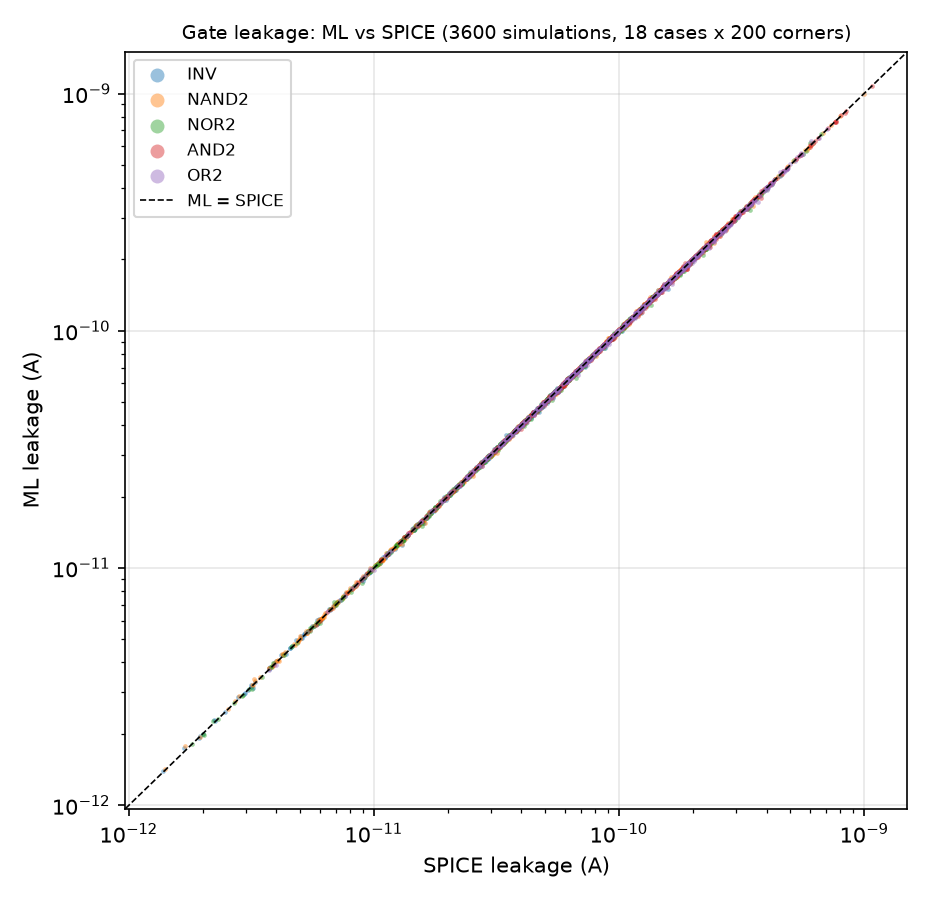
\includegraphics[width=0.75\textwidth]{gate_parity_plot.png}
\caption{Gate parity plot: ML leakage against SPICE leakage for all 3,600 gate simulations (log
axes).}
\end{figure}

\subsection*{Comment}

All 18 cases are close: the median error is between 0.59\pct\ and 0.87\pct. The most accurate
cases are OR2 with inputs 11 and 10 and NAND2 with input 10 (0.59--0.60\pct). The least accurate
are NAND2 with input 11 (0.87\pct), AND2 with input 11 (0.82\pct), and INV with input 0 and NAND2
with input 00 (0.78\pct). The cases with all inputs high are the ones where the ON NMOS gate
tunnelling current is largest, and that current is the least accurate of the ON-state predictions.
The bias is small and positive everywhere (0.14\pct\ to 0.67\pct).

% ==================================================================
\section{Test-circuit results}
% ==================================================================

\subsection*{Circuit}

The 3-bit CLA uses only the Part B gates. With $g_i = a_i b_i$ and $p_i = a_i \oplus b_i$:
\begin{align*}
c_1 &= g_0 + p_0 c_0, \qquad
c_2 = g_1 + p_1 g_0 + p_1 p_0 c_0, \\
c_3 &= g_2 + p_2 g_1 + p_2 p_1 g_0 + p_2 p_1 p_0 c_0, \qquad
s_i = p_i \oplus c_i .
\end{align*}
Each XOR is four NAND2. The circuit has 42 gates (24 NAND2, 12 AND2, 6 OR2) and 204 transistors,
with 7 inputs ($a_0$--$a_2$, $b_0$--$b_2$, $c_0$), so 128 input vectors. The netlist is
\texttt{netlists/circuit/CLA3.cir}.

\subsection*{Method}

\begin{itemize}
\item \textbf{SPICE:} the complete transistor netlist, all 128 input vectors at the same 200
corners as Part B: 25,600 operating points. Points that fail inside a batch run are rerun on their
own (one needed this), so all 25,600 converge. The sum and carry outputs are logically correct in
every simulation.
\item \textbf{ML:} for each input vector a logic simulation gives the inputs of every gate. The
Part B gate model is evaluated for each of the 42 gates at that corner, and the gate leakages are
summed.
\end{itemize}

\subsection*{Results}

\begin{table}[H]
\centering
\small
\begin{tabularx}{\textwidth}{@{}Lcccccc@{}}
\toprule
 & SPICE median (A) & ML median (A) & Bias\,\% & Median err.\,\% & p95 err.\,\% & Mean err.\,\% \\
\midrule
All 25,600 points & 4.539e-09 & 4.555e-09 & 0.59 & 0.74 & 1.79 & 0.80 \\
Most accurate vector (A=011 B=100 Cin=0) & 4.603e-09 & 4.618e-09 & 0.60 & 0.70 & 1.72 & 0.79 \\
Least accurate vector (A=010 B=101 Cin=1) & 4.939e-09 & 4.951e-09 & 0.59 & 0.77 & 1.88 & 0.83 \\
\bottomrule
\end{tabularx}
\end{table}

The mean accuracy is \textbf{99.20\pct}. The circuit leakage ranges from $2.1 \times 10^{-10}$\,A
to $2.6 \times 10^{-8}$\,A over the corners. The table for all 128 input vectors is
\texttt{results/tables/circuit\_results\_table.csv}.

\begin{figure}[H]
\centering
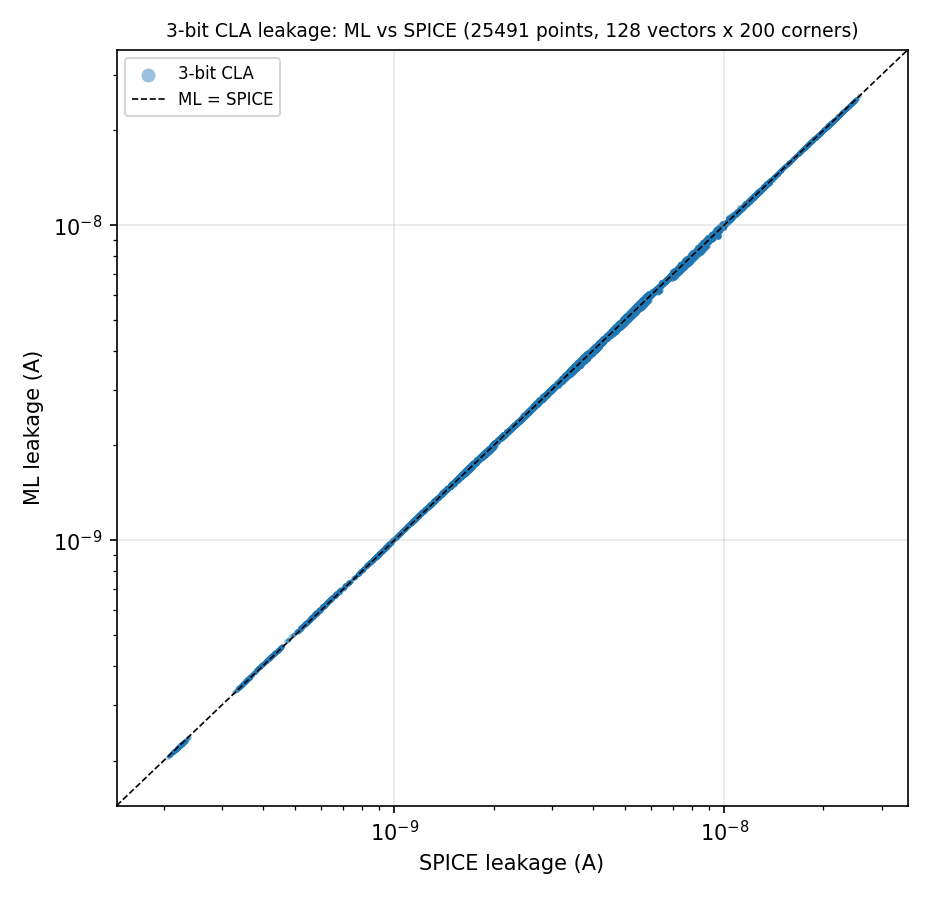
\includegraphics[width=0.75\textwidth]{circuit_parity_plot.png}
\caption{Test-circuit parity plot: ML leakage against SPICE leakage of the 3-bit CLA for all
25,600 operating points (log axes).}
\end{figure}

\subsection*{Comparison with the gate level}

\begin{table}[H]
\centering
\begin{tabular}{@{}lcccc@{}}
\toprule
 & Median err.\,\% & p95 err.\,\% & Mean err.\,\% & Bias\,\% \\
\midrule
Gates (Part B) & 0.69 & 2.07 & 0.83 & 0.46 \\
3-bit CLA (Part C) & 0.74 & 1.79 & 0.80 & 0.59 \\
\bottomrule
\end{tabular}
\end{table}

The circuit accuracy is about the same as the gate accuracy; it is not noticeably lower, as the
specification anticipates. Two reasons:
\begin{itemize}
\item \textbf{Composition costs almost nothing here.} Adding the SPICE leakages of the 42
standalone gates reproduces the SPICE leakage of the whole circuit to 0.002\pct\ (median) and
0.012\pct\ (95th percentile). Internal nodes sit within microvolts of the rails, and counting the
current into high inputs as part of each gate's leakage makes the gate leakages add up exactly.
\item \textbf{Errors neither grow nor average out.} All 42 gates share the same corner, so the same
transistor-model error appears in every gate and carries through to the sum. The spread across
input vectors is small (0.70--0.77\pct), and the 95th percentile is slightly lower than for single
gates because the sum mixes several gate types.
\end{itemize}

% ==================================================================
\section{Error analysis}
% ==================================================================

\begin{itemize}
\item \textbf{Transistor level.} The largest relative errors are in the OFF-state gate current
(median 4.9\pct\ for NMOS, 1.3\pct\ for PMOS; 95th percentile up to 22.8\pct). That current is
about $10^{-22}$\,A and has no effect on leakage. Among currents that matter, the ON-state gate
tunnelling current is the hardest (0.6\pct\ median, 2.5--2.7\pct\ at the 95th percentile): it
depends exponentially on \texttt{toxe} and on both $V_{gs}$ and $V_{gd}$.
\item \textbf{What sets the gate accuracy.} In this low-power technology most of the gate leakage
is gate tunnelling through the ON transistors. For the INV at one corner (VDD 1.10\,V,
30\,\textdegree C), the ON PMOS tunnelling current is $3.7 \times 10^{-11}$\,A and the OFF NMOS
subthreshold current is $5.3 \times 10^{-12}$\,A. So the gate error follows the ON-state $I_g$
error.
\item \textbf{By corner.} At the gate level the median error is 0.81\pct\ below 0\,\textdegree C,
0.76\pct\ from 0 to 60\,\textdegree C and 0.54\pct\ above 60\,\textdegree C; the 95th percentile
is highest below 0\,\textdegree C (2.7\pct). By supply voltage, the 95th percentile is highest for
VDD above 1.03\,V (2.5\pct, against 1.8--1.9\pct\ lower down). The ten largest single gate errors
(4.5--5.9\pct) are at hot, high-VDD corners (corner 74: 113\,\textdegree C, 1.098\,V; corner 83:
97\,\textdegree C, 1.096\,V) and at cold corners (corner 40: $-17.5$\,\textdegree C) where the
leakage is only a few pA.
\item \textbf{By gate and input.} Cases with all inputs high (NAND2 11, AND2 11) are slightly
worse, as noted in the gate results. In the circuit, the largest errors (about 4\pct) are again
all at corner 74.
\item \textbf{Why the gate operating points matter.} Before they were added to the training data,
the same models gave a 26--46\pct\ mean gate error with a steady negative bias, although their
test-set errors were about 1\pct. The ON transistors in a gate have $V_d \approx V_s$ and a full
$V_{gs}$, which is the corner of the sampled $(V_d, V_s)$ square, and the ML corrections were
extrapolating there.
\item \textbf{SPICE reference.} A few gate simulations converged to a non-physical solution (an
internal node above VDD) with a leakage about 100 times too high, and one (AND2, input 00, corner
4) did not converge with ngspice's default sparse solver. These are rerun with a different
starting guess and then with the KLU solver, after which all 3,600 are valid.
\end{itemize}

% ==================================================================
\section{Limitations and improvements}
% ==================================================================

\begin{itemize}
\item \textbf{A systematic bias remains} (+0.5\pct\ at the gates, +0.6\pct\ in the circuit).
Because every gate in a circuit shares the corner, this bias does not average out. More samples at
gate operating points, or a better tunnelling equation with the BSIM4 $I_{gc}$ partition between
source and drain, should reduce it.
\item \textbf{The training data is tuned to gates.} 20\pct\ of the samples are gate operating
points, so the dataset is no longer purely uniform. The models are most accurate where gates
operate and less so in parts of the $(V_d, V_s)$ range that gates do not use.
\item \textbf{The models need BSIM4's internal current components for training.} These come free
from the same simulations, but a different simulator or model card may not expose them.
\item \textbf{Drain and source junction areas are left at their defaults} (as in the TA's example
netlist), which gives the drain junction a fixed $10^{-14}$\,A saturation current. With real
layout areas the junction leakage would change and the models would need retraining.
\item \textbf{Part B uses node voltages from SPICE,} as the specification asks. The models can also
solve the internal nodes themselves with no loss of accuracy, so a SPICE-free flow is possible;
this was verified only for the five gates here.
\item \textbf{The circuit method assumes rail-to-rail gate inputs.} That holds for this static CMOS
adder (the composition error is 0.002\pct), but not for circuits with pass transistors or degraded
logic levels.
\item \textbf{Only DC leakage at fixed input vectors is covered.} Larger circuits would need the
input vectors sampled instead of enumerated.
\end{itemize}

% ==================================================================
\section{Deliverables and reproduction}
% ==================================================================

\begin{table}[H]
\centering
\small
\begin{tabularx}{\textwidth}{@{}p{4.2cm}L@{}}
\toprule
Deliverable & Location in the repository \\
\midrule
Datasets & \texttt{data/transistor/<CASE>.csv} (four files, 10,000 rows each) \\
Example netlists & \texttt{netlists/transistor}, \texttt{netlists/gates}, \texttt{netlists/circuit/CLA3.cir} \\
Data check & \texttt{results/tables/kirchhoff\_check.csv}, \texttt{results/plots/trend\_*.png} \\
Model comparison table & \texttt{results/tables/model\_comparison.txt}, \texttt{model\_comparison\_validation.csv} \\
Chosen models & \texttt{results/tables/chosen\_models\_test.csv}, \texttt{results/plots/pred\_vs\_spice\_*.png}, \texttt{ml\_models/<CASE>.joblib} \\
Gate results and parity plot & \texttt{results/tables/gate\_results\_table.csv}, \texttt{results/plots/gate\_parity\_plot.png} \\
Test-circuit results & \texttt{results/tables/circuit\_results\_table.csv}, \texttt{results/plots/circuit\_parity\_plot.png} \\
Code & \texttt{scripts/01\_*.py} to \texttt{scripts/05\_*.py}, seeds in \texttt{scripts/config.py} \\
\bottomrule
\end{tabularx}
\end{table}

The scripts are run in order; set the environment variable \texttt{NGSPICE} to the ngspice console
executable if it is not on the path.

\begin{verbatim}
python scripts/01_generate_transistor_data.py   # Part A step 1 (~3 min)
python scripts/02_check_transistor_data.py      # Kirchhoff check and trend plots
python scripts/03_train_transistor_models.py    # Part A step 2 (~25 min)
python scripts/04_gate_validation.py            # Part B (~6 min)
python scripts/05_circuit_validation.py         # Part C (~60 min)
\end{verbatim}

All random draws use fixed seeds set in \texttt{scripts/config.py}. A full rerun reproduces the
datasets bit for bit and the results above.

\end{document}
